\begin{figure}[H]
    \centering
    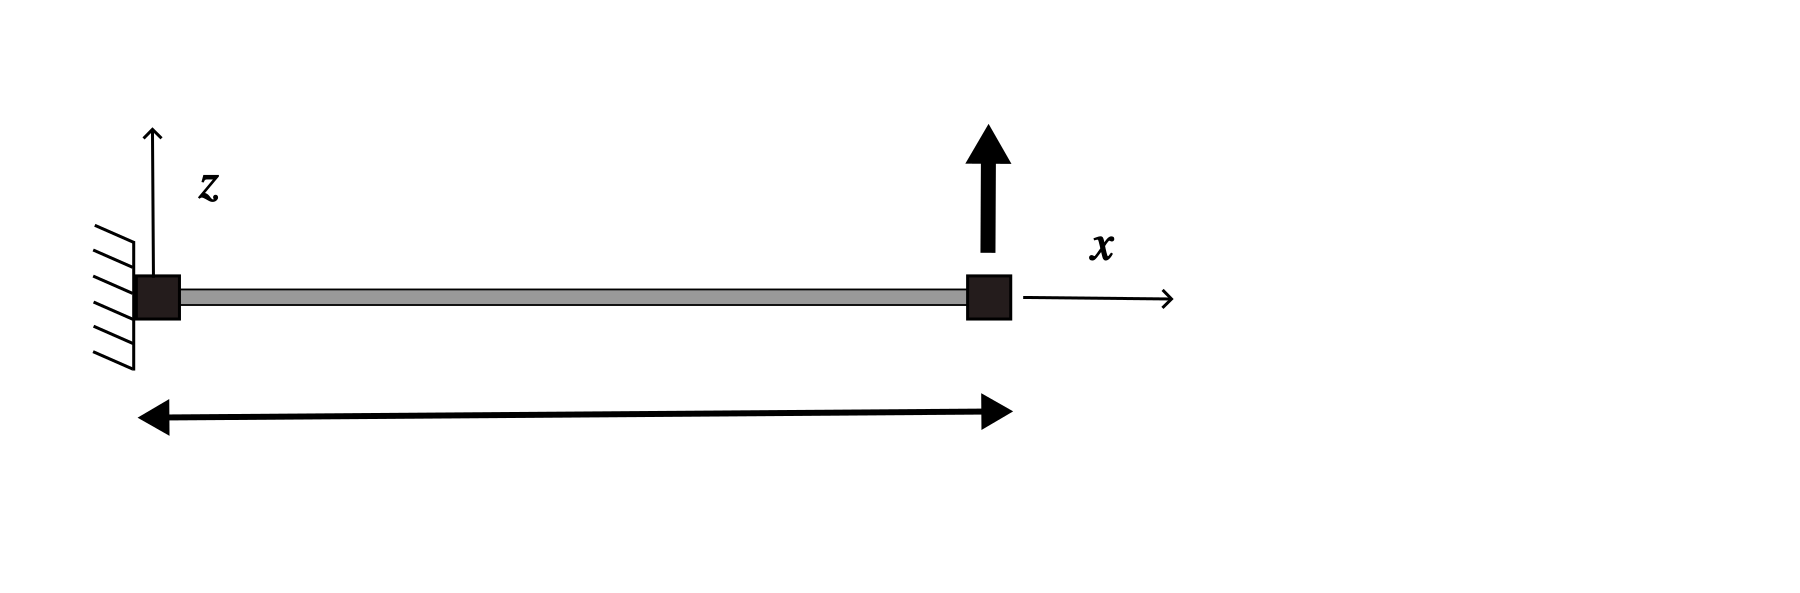
\includegraphics[width=0.5\linewidth]{Examples/frame-1020/img/frame-1020.png}
    \caption{Model for Example~\ref{sec:frame-1020}.}
    \label{fig:1020}
\end{figure}

\subparagraph{Context}
This problem demonstrates the capability to simulated follower nodal loads. The problem was considered by \cite{simo1986threedimensional}.

\subparagraph{Setup}
A cantilever is subjected to a transverse follower force at its tip. 


\FrameSection{
label/problem=frame-1020,
unit/length={\milli\meter},
A=1.61538e8,
Iz=3.5e7,
Iy=3.5e9
}

\subparagraph{Results}
Tip deflections are plotted in \cref{fig:1020-disp}. 
Both the \ExactFrame{} and \ForceFrame{} with \Corotational{} geometry perform well. 

\begin{figure}[H]
    \centering
    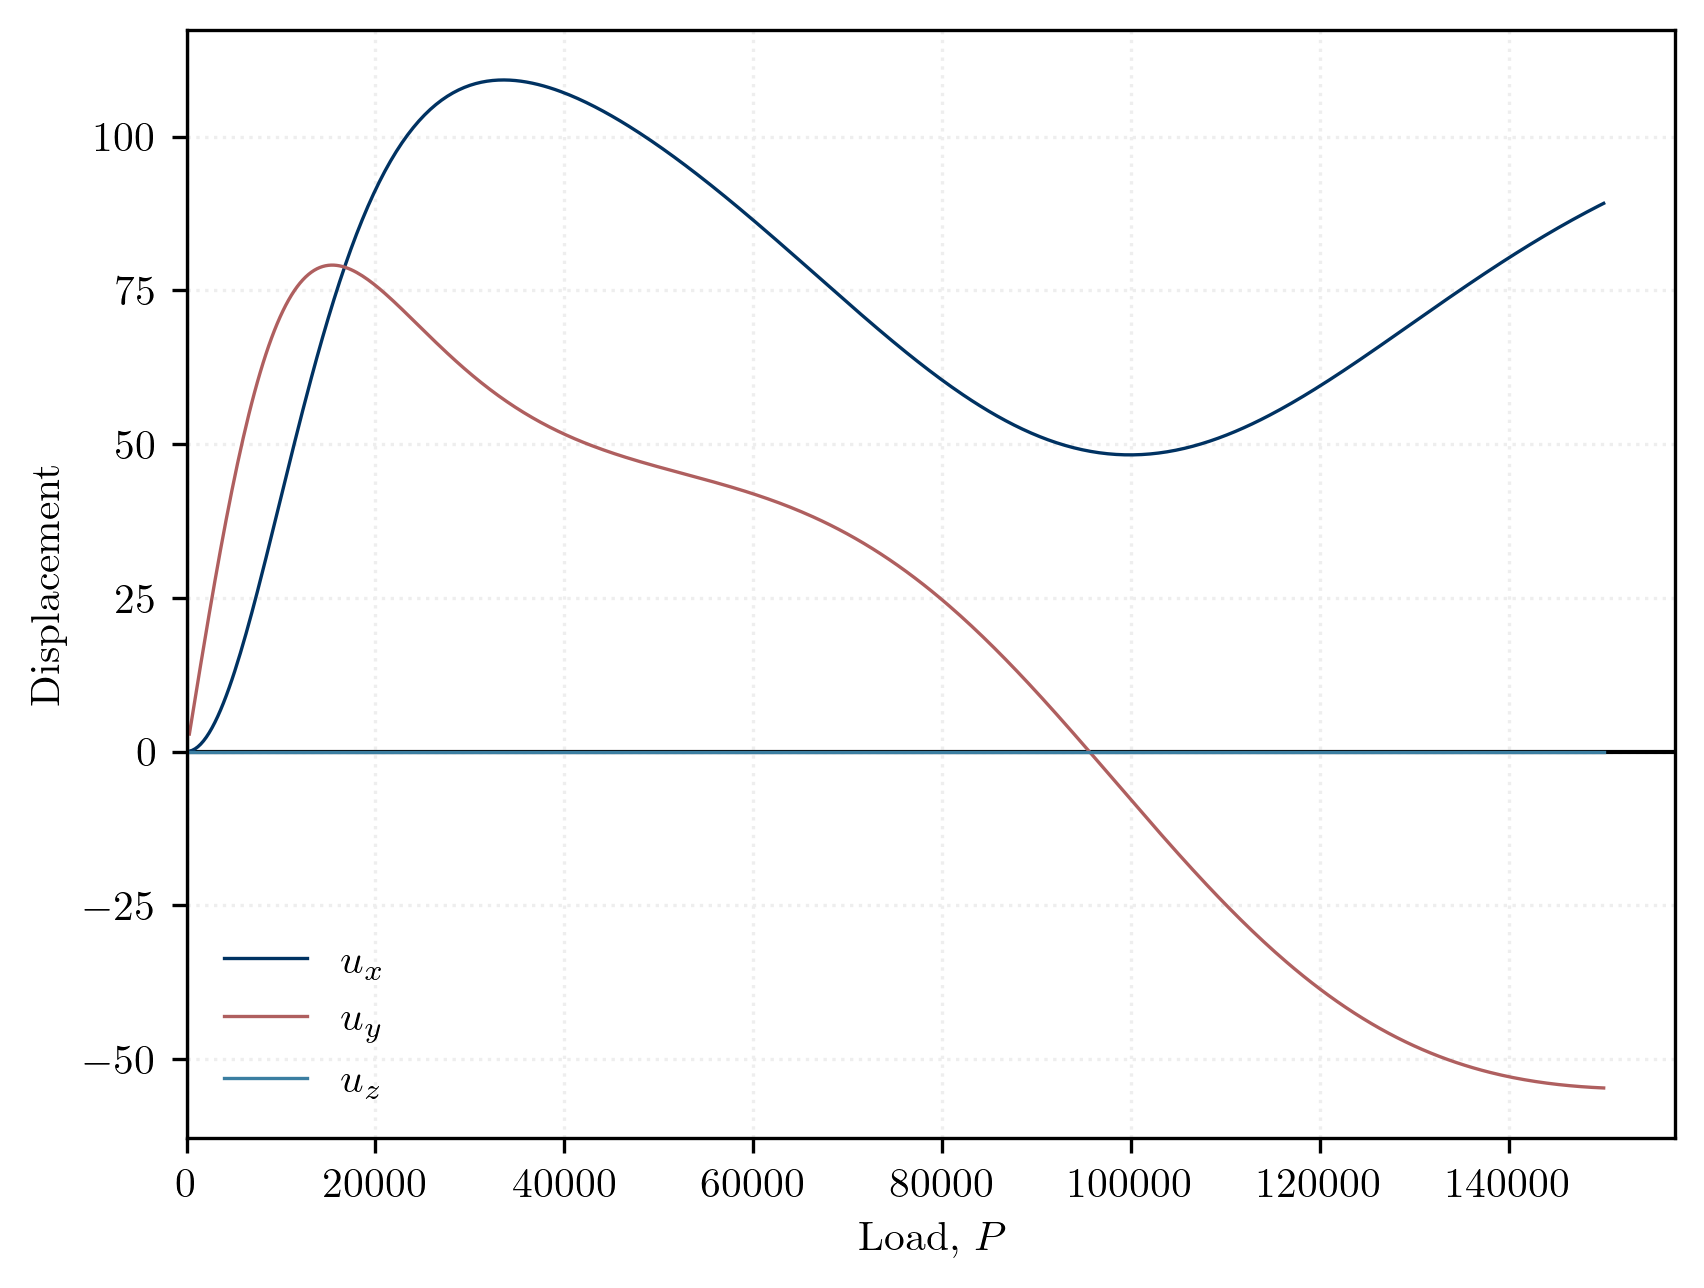
\includegraphics[width=0.6\linewidth]{Examples/frame-1020/img/1020-Exact-displacement.png}
    \caption{Displacements for a cantilever under a transverse follower load (Example~\ref{sec:frame-1020}).}
    \label{fig:1020-disp}
\end{figure}

\subparagraph{Conclusions}

